\section*{Results}

The synchronization time delay between two nodes was tested, focusing on the initial schedule delay. Figure 4 shows the time delay between the start of the active phase in each cycle. This experiment was done across three sessions with varying initialization delays. In all sessions, nodes were active for 3 seconds and slept for 15 seconds. The synchronization phase was triggered every 4 cycles. The results indicate that if the initial delay is small, the nodes achieve near-synchronization after the first synchronization phase, with a delay of less than 4 ms. However, if the nodes have significantly different initial schedules, synchronization takes longer, with the worst case showing synchronization only after 17 cycles. Once synchronized, the nodes maintain this state.

\begin{figure}[h]
\centering
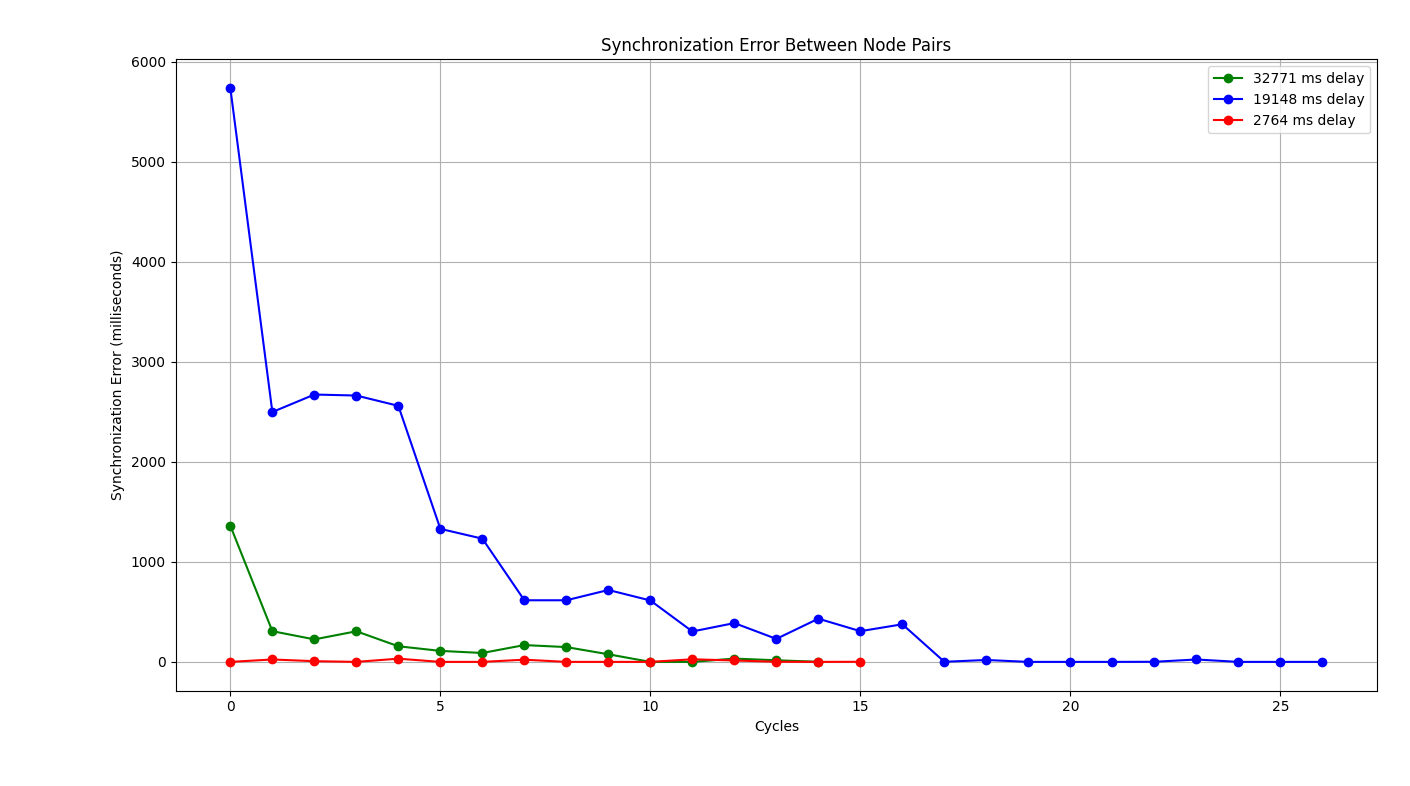
\includegraphics[width=0.9\textwidth]{figures/sync-error.png}
\caption{Synchronization Error}
\end{figure}

Additionally, the number of cycles required to successfully transfer 5 packets with varying payload sizes in a unicast communication setup was tested. For this test, the sleeping duration was set to 8 seconds, the active duration to 3 seconds, the synchronization phase to 200 cycles, and packet dropping was disabled. The results, shown in Figure 5, were not good. It took 3 cycles (33 seconds) to send 5 packets with a 5-byte payload and 19 cycles (almost 3.5 minutes!) for a 180-byte payload. This poor performance is due to the 1\% duty cycling rule and packet loss. A CSMA approach might have improved the efficiency of packet transmission and reception.

\begin{figure}[h]
\centering
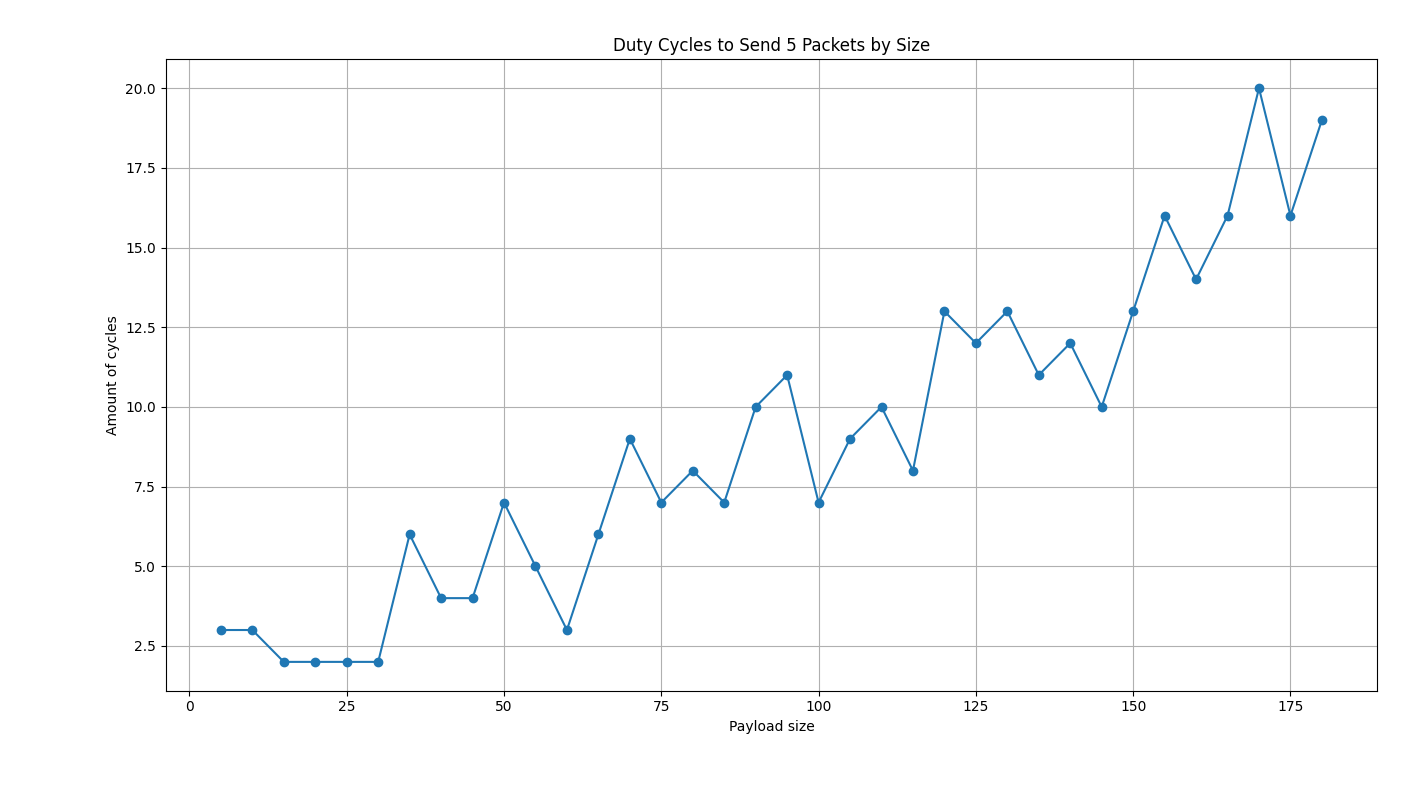
\includegraphics[width=0.9\textwidth]{figures/packet-loss.png}
\caption{Cycles needed to send 5 packets of varying size}
\end{figure}
